\section{Attenuation Models}

In physics-based ground motion simulation, $Q$ is considered as a user-defined value. Community velocity models ($CVMs$) used in simulations do not generally provide values of $Q$. Such a high resolution $Q$ model requires a rigorous inversion process. Therefore, the value of \qs{}, for instance, is usually defined based on rules that depend on the value of \vs{}. Typical forms of \qsvs{} relationships are (piecewise) linear or polynomial functions \citep[e.g.,][]{Brocher_2008_BSSA, Brocher_2005_Tech,Olsen_2003_BSSA, Graves_2008_BSSA,Taborda_2013_BSSA}. The value of \qp{} is mostly defined in terms of \qs{}, and, in some cases, also on the velocity contrast, $V_{P}/V_{S}$. Table~\ref{tab:QsVstable} shows a collection of different \qsvs{} and \qpqs{} relationships used in simulations and other related studies, including the earthquake or scenario event for which they were employed, and the simulation's minimum shear wave velocity (\vsmin{}) and maximum frequency (\fmax{}). Fig.~\ref{fig:Figure_q_models}  shows the \qs{} values with respect to \vs{} for each \qsvs{} relationship.  

% Please add the following required packages to your document preamble:
% \usepackage{multirow}
\begin{table}[]
	\centering
	\caption{Examples of \qsvs{} and \qpqs{} relationships used in past physics-base simulations}
	\label{tab:QsVstable}
	\renewcommand{\arraystretch}{0.75}
	\resizebox{\textwidth}{!}{%
		\begin{tabular}{lccccccc}
			\textbf{Publication}                                                        		    & \textbf{Simulation}                                       &  \textbf{\vsmin{}}             & \textbf{\fmax{}}                          & \multicolumn{3}{c}{\textbf{\qs{}=g(\vs{})}}                     &\textbf{\qp{}=h(\qs{})}                                 \\ 
			                                                                                       		    &                                                                     &  \textbf{(m/s)    }             & \textbf{(Hz)}                                 & \multicolumn{3}{c}{\textbf{($V_{S}$ in km/s, depth $z$ in km)}}         &                               \\ \hline
			\citet{Olsen_2003_BSSA}                                             		    & 1994 Northridge                                          & \multirow{2}{*}{500}        & \multirow{2}{*}{0.5}                    & 20\vs{}                                                             &   & \vs{}$< 1.5$                           & \multirow{2}{*}{1.5\qs{}} \\ 
			\citet{Olsen_2008_BSSA}                                              		    & TeraShake$$                                               &                                        &                                                   & 100\vs{}                                                           &   & \vs{} $\geq 1.5$                       &                            \\\hline
			\citet{Olsen_2009_GRL}                                               		    & ShakeOut                                                    & \multirow{3}{*}{500}        & \multirow{3}{*}{0.5}                    & \multicolumn{3}{c}{\multirow{4}{*}{50\vs{}}}     & \multirow{4}{*}{2\qs{}}                             \\
			\citet{Bielak_2010_GJI}$^{FD}$                                    		    &  ShakeOut                                                   &                                        &                                                   & \multicolumn{3}{c}{}                                          &                                                 \\
			\citet{Graves_2011_PAG}                                              		    & CyberShake                                                &                                         &                                                  & \multicolumn{3}{c}{}                                          &                                                 \\ \cline{3-4}
			\citet{Cui_2010_Proc}                                                   		    & M8                                                               & 400                                  & 2.0                                            & \multicolumn{3}{c}{}                                          &                                                 \\ \hline
			\multirow{2}{*}{\citet{Komatitsch_2004_BSSA}}             		    & 2001 Hollywood                                          & \multirow{2}{*}{670}         & \multirow{2}{*}{0.5}                   & 90                                 &   & Sediments                              & \multirow{2}{*}{$\infty$}  \\
			                                                                                        		    & 2002 Yorba Linda                                        &                                         &                                                  & $\infty$                           &   & Bedrock                                &                            \\ \hline
			\citet{Taborda_2006}$^\mathsection$                              		    & TeraShake                                                   & 300                                  & 1.0                                            & \multicolumn{3}{c}{\multirow{3}{*}{50\vs{}}}                                                                                  &                                                                 \\
			\citet{Taborda_2007} $^\mathsection$                            	            & ShakeOut                                                    & 200                                  & 1.0                                             & \multicolumn{3}{c}{}                                                                                                                    &                                                                  \\
			\citet{Bielak_2010_GJI}$^{FE,}$$^\mathsection$                            & ShakeOut                                                   & 500                                   & 0.5                                            & \multicolumn{3}{c}{}                                                                                                                    &                                                                 \\ \hline
			\citet{Graves_2008_BSSA}                                    		             & 2001 Big Bear                                            & 250                                   & 1.0                                            & \multicolumn{3}{c}{60\vs{}}                                                                                                           &                                                 \\ \cline{5-7}
			\multirow{3}{*}{\citet{Aagaard_2008_BSSA}}            			     & \multirow{3}{*}{1989 Loma Prieta}             & \multirow{3}{*}{330-760}   & \multirow{3}{*}{0.5-1.0}             & $50V_{S}$         &   & $V_{S}< 0.9$                           & \multirow{6}{*}{$2$\qs{}}  \\
			                                                                                    		  	     &                                                                    &                                         &                                                   & $60 V_{S}^{1.5}$                   &   & $0.9 \leq V_{S}<3.4$                   &                            \\
			                                                                                       		     &                                                                    &                                         &                                                  & $500$                              &   & $3.4 \geq V_{S}$                       &                            \\ \cline{5-7}
			\multirow{3}{*}{\citet{Brocher_2008_BSSA}$^\mathparagraph$}     &                                                                     &                                        &                                                   & 13                                 &   & $V_{S}<0.3$                            &                            \\
			                                                            					    &                                                                     &                                         &                                                   & $-16+104.13V_{S}$                  &   & \multirow{2}{*}{$0.3\leq V_{S} < 5.0$} &                            \\
			                                                            					    &                                                                     &                                         &                                                   & $-25.225{V_{S}}^2+8.2184{V_{S}}^3$ &   &                                        &                            \\ \hline
			\citet{Chaljub_2010_BSSA}$^\dagger$                                           & 2003 Lancey, and                                        & \multirow{2}{*}{300}        & \multirow{2}{*}{2.0}                     & 50                                 &   & $z<1$                                  & $3/4(V_{P}/V_{S})^2Q_{S}$  \\
			                                                            				            & Event S1                                                      &                                        &                                                    & $\infty$                           &   & $z\geq1$                               & $\infty$                   \\ \hline
			\citet{Taborda_2013_BSSA}                                    			    & \multirow{2}{*}{2008 Chino Hills}                 & \multirow{2}{*}{200}        & \multirow{2}{*}{4.0}                     & \multicolumn{3}{c}{\multirow{3}{*}{\begin{tabular}[c]{@{}c@{}}$10.5 - 16V_{S} + 153 V_{S}^2-103V_{S}^3$\\ $+ 34.7V_{S}^4-5.29*V_{S}^5+0.31V_{S}^6$\end{tabular}}} & \multirow{3}{*}{$3/4(V_{P}/V_{S})^2Q_{S}$} \\
			\citet{Taborda_2014_BSSA}                                    			    &                                                                     &                                        &                                                    & \multicolumn{3}{c}{}                                                                                                                        &                                                 \\ \cline{1-4}
			\citet{Taborda_2016_GJI}                                                                & 30 earthquakes                                           & 200                                  & 1.0                                              & \multicolumn{3}{c}{}                                                                                                                        &                                                 \\ \hline
			\citet{Withers_2015_BSSA}$^\ddagger$                                         & 2008 Chino Hills                                         & 200                                  & 4.0                                               & \multicolumn{3}{c}{$100V_{S}$}                                                                                                       & $2$\qs{}                                              \\ \hline
			\multicolumn{4}{l}{$*$ Denotes scenario events}                                                                                & \multicolumn{4}{l}{$\dagger$ Simulations for Grenoble Valley, France}                                                                                                                                                                                                                   \\
			\multicolumn{4}{l}{$\mathsection$ Rayleigh damping instead of a visco-elastic model}                     & \multicolumn{4}{l}{$^{FE}$ Finite-element simulation results therein}                                                                                                                                                                                                                 \\
			\multicolumn{4}{l}{$\mathparagraph$ Empirical relations (no simulation) for Northern California}     & \multicolumn{4}{l}{$^{FD}$ Finite-difference simulation results therein}            \\
			\multicolumn{4}{l}{$\ddagger$ Frequency independent part of $Q$}                                                  & \multicolumn{4}{l}{}                                                                                                                                                                                                     
		\end{tabular}}
\end{table}

 \begin{figure}
    \centering
    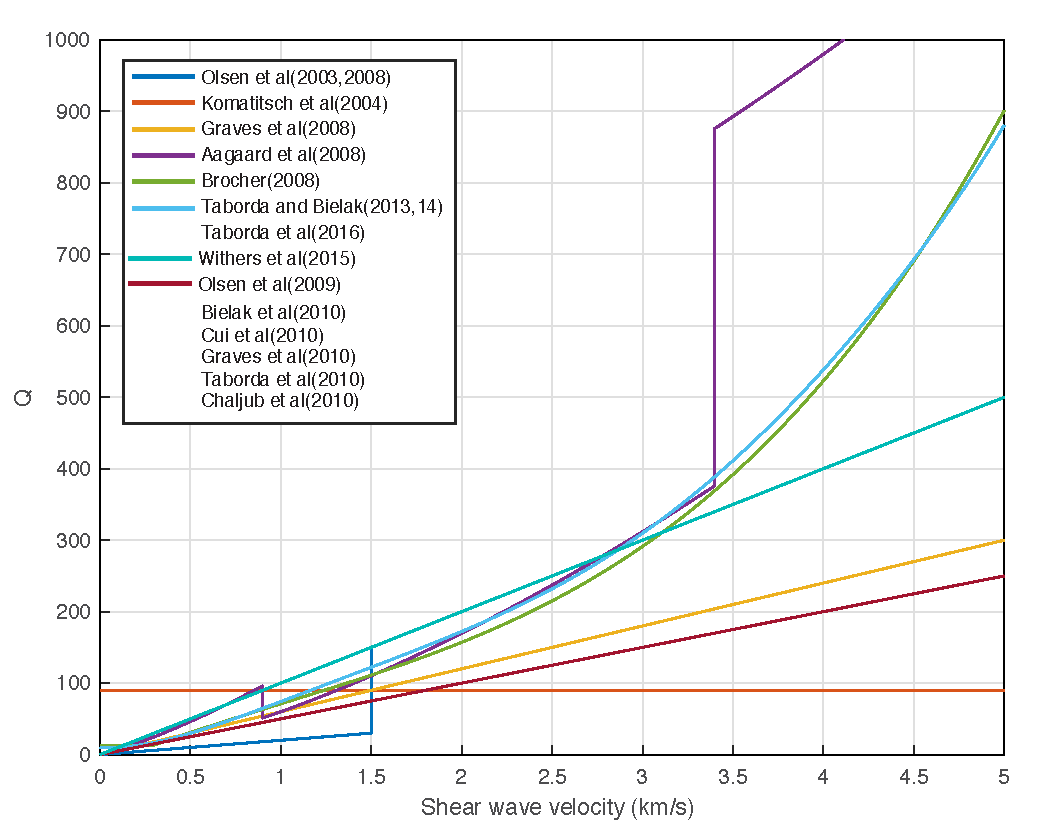
\includegraphics[width=400 px]{figures/pdf/Figure_01.pdf}
    \caption{Illustration of \qsvs{} relationships introduced in Table~\ref{tab:QsVstable}.}
    \label{fig:Figure_q_models}
\end{figure}

This figure illustrates the significant differences between these models. There is no consensus on the most appropriate set of relationships between seismic velocities and quality factors. The relationship used by \citet{Taborda_2013_BSSA} was introduced as an attempt to capture some of the main features of other \qsvs{} rules. It is known that the relationships between \qs{} and \vs{}, and between \qp{} and \qs{} can be depth dependent (see, for instance, \citet{Olsen_2003_BSSA}, and the references therein) although \qs{} remains strongly correlated with \vs{}.  \citet{Hauksson_2006_JGR} also show that while \qs{} and \qp{} increase rapidly with depth consistent with the crustal structure, but argue that the ratios between \qs{} and \qp{} vary with depth and are different within and outside the major basins in southern California. They obtained values of \qsoqp$>1$ for most of the region but found a few limited areas, mostly outside the major sedimentary basins, where \qsoqp$< 1$. \citet{Song_2013_AGU} concluded that, in general, $Q_{S} \geq Q_{P}$, with $Q_{S} \approx Q_{P}$ near the surface $(z < 5 km)$ but $Q_{S} > Q_{P}$ at depth; and indicated that \qs{} seems to be in better agreement with the rule $Q_{S} = 50V_{S}$ at depth but not near the surface, where \qs{} is not linearly related to \vs{}. However, most of the simulations done recently (as seen in Table.~\ref{tab:QsVstable}) correspond to numerical models with maximum frequencies, \fmax{} $\leq1-2$~Hz, and minimum shear wave velocities, \vsmin{}$\geq300$~ m/s, where one can still assume $Q$ to be frequency independent. 




